\section{Tuesday, September 5, 2023}

\subsection{More on Conditional Statements}
With conditional statements, we can expand them into different archetypes to create more basis for logical equivalencies. We call these the \vocab{converse, inverse, }and \vocab{contrapositive}.

\subsubsection{Converse}
The converse of a logical statement is more or less just re-arranging the statement variables so that they are reversed. Therefore, the converse of a statement:
\begin{displaymath}
    p \rightarrow q
\end{displaymath}
is expressed as:
\begin{displaymath}
    q \rightarrow p
\end{displaymath}

Of course, from this it would be pretty intuitive to say that the converse is \textbf{not} logically equivalent to the original statement.

\subsubsection{Contrapositive}
The contrapositive of a logical statement is practically just the negation of a converse, or using DeMorgan's law (only on the statement variables) of the converse. Therefore, the contrapositive of a logical statement is:
\begin{displaymath}
    p \rightarrow q
\end{displaymath}
is expressed as:
\begin{displaymath}
    \neg q \rightarrow \neg p
\end{displaymath}

This would mean that the original statement and the contrapositive of that statement \textbf{are} logically equivalent.

\subsubsection{Inverse}
The inverse of a logical statement is the negation of the original statement itself. Therefore, the inverse of a logical statement can be shown as:
\begin{displaymath}
    p \rightarrow q
\end{displaymath}
being:
\begin{displaymath}
    \neg p \rightarrow \neg q
\end{displaymath}

\subsection{Biconditionals}
In logic, we can treat implications where it can be described as an "if any only if" statement as a \vocab{biconditional}. Portrayed through the truth table, we can see:

\begin{displaymath}
    \begin{array}{|c|c|c|}
    p & q & p \iff q\\ 
    \hline
    T & T & T\\
    T & F & F\\
    F & T & F\\
    F & F & T\\
    \end{array}
\end{displaymath}

The biconditional also has its own logical equivalence, considering it the tautology:

\begin{displaymath}
    p \iff q \equiv (p \rightarrow q) \land (q \rightarrow p)
\end{displaymath}

\subsubsection{Necessary and Sufficient Conditions}
Suppose we have statements p and q in a biconditional. We can distinguish two different conditions for p and q depending on how the whole statement is written.

\begin{itemize}
    \item p is a sufficient condition for q means, if p then q.
    \item p is a necessary condition for q means if not p then not q.
\end{itemize}

\subsection{Arguments and Rules of Inference}
\textbf{\underline{Definition 3.1}}: An \vocab{argument} is a conjecture that say that if you make certain assumptions, then a particular statement must follow.

\begin{itemize}
    \item The assumptions are called \vocab{premises}.
    \item The statement that follows is the \vocab{conclusion.}
\end{itemize}

An argument is considered valid when, for all interpretations that make the premises true, the conclusion is also true.

Recall the laws of logical equivalencies.

\vspace{0in}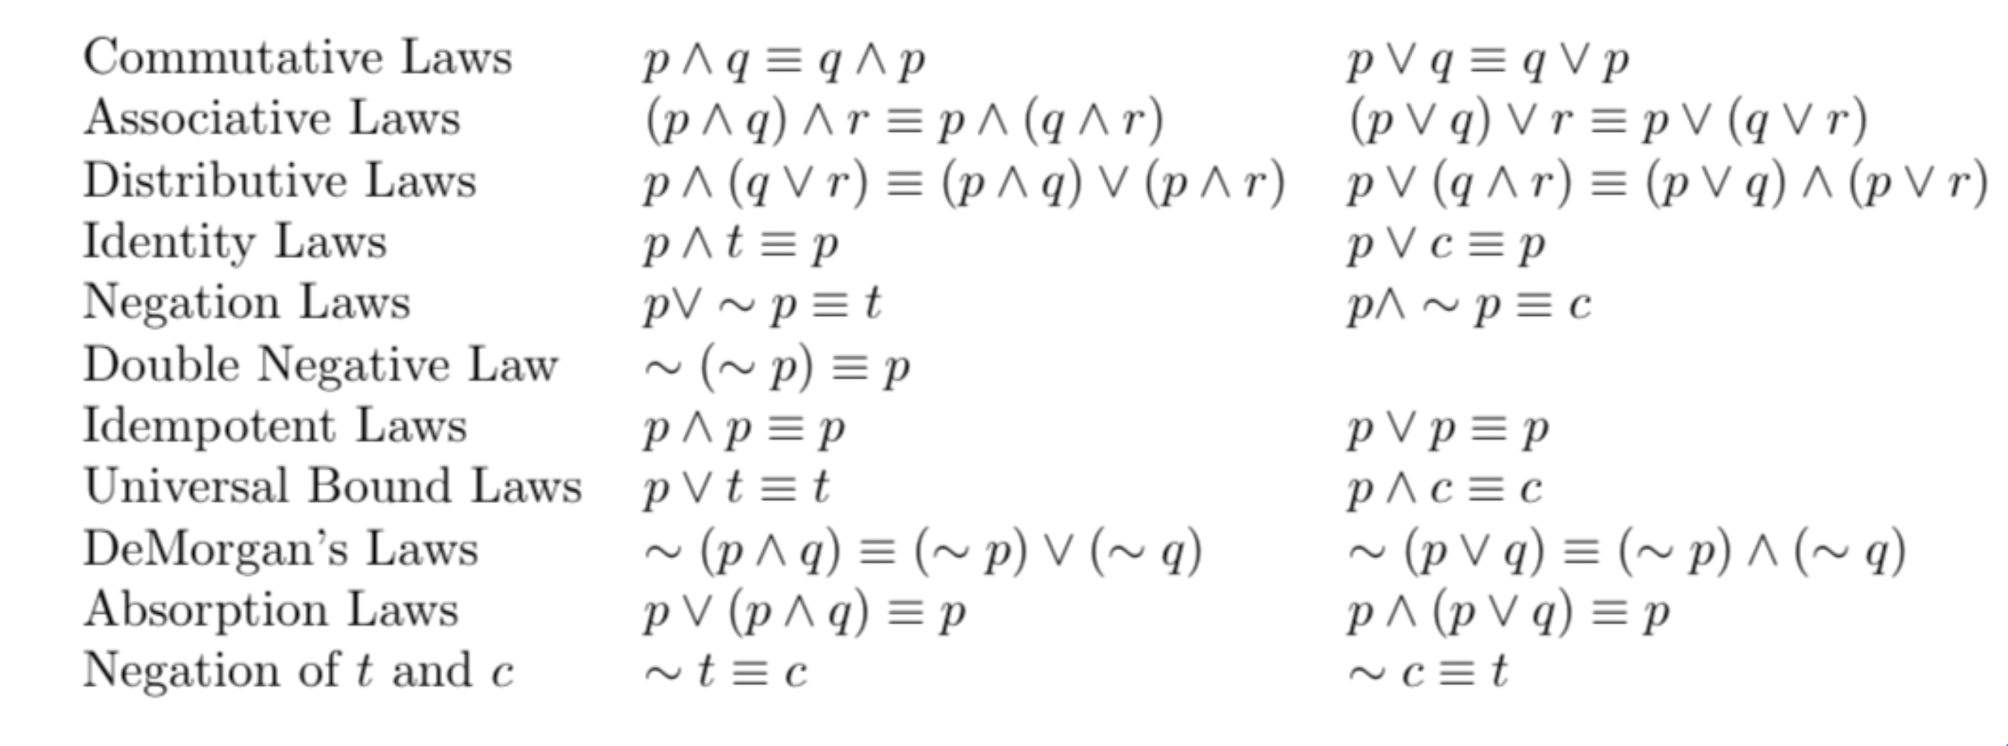
\includegraphics[scale=0.4]{media/commonlogicalequivalencies.png} 

We can use these in proving arguments, alongside our new friend, the \vocab{rules of inference}. We can use these rules of inference to prove the validity of complex arguments.

\vspace{0in}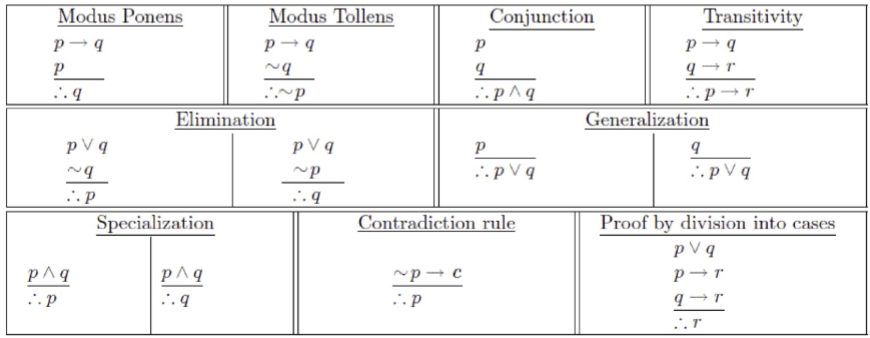
\includegraphics[scale=1]{media/Screenshot 2023-10-02 at 5.51.13 PM.png} 

\begin{example}
$p \iff q$\\
$q \rightarrow r$\\
$p \lor s$\\
$\neg r$\\
$\therefore s$
\end{example}

Using logical equivalence and rules of inference, we can prove this pretty easily.

\begin{logicproof}{1}
p \iff q & Premise\\
q \rightarrow r & Premise\\
p \lor s & Premise\\
\neg r & Premise\\
(p \rightarrow q) \land (q \rightarrow p) & Definition of Biconditional of 1\\
p \rightarrow q & Specialization of 5\\
q \rightarrow p & Specialization of 5\\
p \rightarrow r & Transitivity of 2 and 7\\
\neg p & Modus Tollens of 8 and 4\\
s & Elimination of 3 and 9
\end{logicproof}